% !TEX root = task-7-2.tex
% Editable task bank. Append new BankTask blocks at the end of the document.
\documentclass[12pt,a4paper]{article}
\usepackage{physics-textbook}
\usepackage{graphicx,needspace}
\usetikzlibrary{decorations.pathmorphing}
\newif\ifShowSolutions
\ifdefined\TutorEdition
  \ShowSolutionstrue
\else
  \ShowSolutionsfalse % Change to \ShowSolutionstrue to display solutions.
\fi
\newcounter{banktask}
\newsavebox{\BankTaskBox}
\newcommand{\BankTaskContent}[3]{%
  \noindent\textbf{\thebanktask.}\quad #2\par
  \ifShowSolutions
    \Needspace{50mm}% Keep the solution heading with its opening text or diagram.
    #3\par
    \ifdefined\TutorEdition
      \ifcsname TutorSource#1\endcsname
        \nopagebreak\smallskip{\small\csname TutorSource#1\endcsname\par}%
      \fi
    \fi
  \fi
}
\newcommand{\BankTask}[3]{%
  \refstepcounter{banktask}\par\medskip
  \sbox{\BankTaskBox}{\begin{minipage}{\linewidth}%
    \BankTaskContent{#1}{#2}{#3}\end{minipage}}%
  \ifdim\dimexpr\ht\BankTaskBox+\dp\BankTaskBox\relax>\dimexpr\textheight-20mm\relax
    \Needspace{35mm}\BankTaskContent{#1}{#2}{#3}%
  \else
    \Needspace{\dimexpr\ht\BankTaskBox+\dp\BankTaskBox\relax}%
    \noindent\usebox{\BankTaskBox}\par
  \fi
  \medskip
}
\begin{document}
\BookSubsection{7.2}{Измерения и погрешности}


% Source F13F4D: https://ege.fipi.ru/bank/questions.php?search=1&proj=BA1F39653304A5B041B656915DC36B38&qid=F13F4D
\BankTask{F13F4D}{
Чтобы узнать диаметр медной проволоки, ученик намотал её виток к витку на карандаш и измерил длину намотки из \(20\) витков. Длина оказалась равной \((15 \pm 1)\,\text{мм}\). Запишите в ответ диаметр проволоки с учётом погрешности измерений.
}{
\smallskip\noindent\textbf{Решение от GPT}\par
Диаметр проволоки равен длине намотки, делённой на число витков: \(d=\frac{15}{20}=0{,}75\,\text{мм}\). Погрешность диаметра \(\Delta d=\frac{1}{20}=0{,}05\,\text{мм}\). Ответ: \((0{,}75\pm0{,}05)\,\text{мм}\).
}

% Source 2EC822: https://ege.fipi.ru/bank/questions.php?search=1&proj=BA1F39653304A5B041B656915DC36B38&qid=2EC822
\BankTask{2EC822}{
В книге \(250\) листов. По результатам измерения с помощью линейки толщина книги составляет \(3{,}5\,\text{см}\). Чему равна толщина одного листа по результатам этих измерений, если погрешность линейки равна \(\pm1\,\text{мм}\)?
}{
\smallskip\noindent\textbf{Решение от GPT}\par
Толщина книги \(3{,}5\,\text{см}\) равна \(35\,\text{мм}\), поэтому толщина одного листа \(d=\frac{35}{250}=0{,}140\,\text{мм}\). Погрешность равна \(\Delta d=\frac{1}{250}=0{,}004\,\text{мм}\). Ответ: \((0{,}140\pm0{,}004)\,\text{мм}\).
}

% Source B044CF: https://ege.fipi.ru/bank/questions.php?search=1&proj=BA1F39653304A5B041B656915DC36B38&qid=B044CF
\BankTask{B044CF}{
\(150\) одинаковых болтов, упакованных в пакет, положили на весы. Весы показали \(75\,\text{г}\). Чему равна масса одного болта по результатам этих измерений, если абсолютная погрешность данного измерения равна \(3\,\text{г}\)? Массу самого пакета не учитывать.
}{
\smallskip\noindent\textbf{Решение от GPT}\par
Масса одного болта \(m=\frac{75}{150}=0{,}50\,\text{г}\). Абсолютная погрешность массы одного болта \(\Delta m=\frac{3}{150}=0{,}02\,\text{г}\). Ответ: \((0{,}50\pm0{,}02)\,\text{г}\).
}

% Source EDAAE9: https://ege.fipi.ru/bank/questions.php?search=1&proj=BA1F39653304A5B041B656915DC36B38&qid=EDAAE9
\BankTask{EDAAE9}{
Динамометр с прикреплённым к нему бруском тянут влево, как показано на рисунке. Брусок движется с постоянной скоростью. Абсолютная погрешность измерения силы при помощи динамометра равна цене деления прибора. Запишите значение силы трения скольжения, действующей на брусок, с учётом абсолютной погрешности измерений.
\begin{center}
\begin{tikzpicture}[book diagram,x=1cm,y=1cm]
\draw[line width=1.2pt] (0,0)--(7.7,0);
\foreach \x in {0.1,0.3,...,7.7}{\draw (\x,0)--++(-0.12,-0.15);}
\draw (0,0.3) rectangle (4.2,1.75);
\draw (0.1,0.3)--(0.1,1.75);
\draw (5.5,0.05) rectangle (7.4,1.88);
\draw[-{book tip}] (2.3,2.1)--(0.25,2.1);
\draw (0.1,0.78)--(0.1,0.94);
\draw plot[domain=0:2880,samples=481,variable=\t] ({0.1+3.05*\t/2880+0.13*sin(\t)},{1.04+0.23*cos(\t)});
\draw (3.15,1.27)--(3.25,1.04)--(5.15,1.04);
\draw (5.15,1.04) arc[start angle=180,end angle=500,radius=0.12];
\fill (5.37,1.04) circle (0.065);
\draw (3.25,0.5)--(3.25,1.4);
\draw (1.35,0.3)--(3.85,0.3);
\foreach \i in {0,...,25}{
\pgfmathsetmacro{\xx}{1.35+0.1*\i}
\draw (\xx,0.3)--(\xx,0.43);
}
\foreach \i in {0,...,5}{
\pgfmathsetmacro{\xx}{1.35+0.5*\i}
\draw (\xx,0.3)--(\xx,0.5);
\node[rotate=90,anchor=west,font=\small] at (\xx,0.57) {$\i$};
}
\node[rotate=90] at (0.38,0.59) {$\text{Н}$};
\end{tikzpicture}
\end{center}
}{
\smallskip\noindent\textbf{Решение от GPT}\par
При постоянной скорости сила трения равна силе тяги: $F_{\text{тр}}=F_{\text{дин}}$. Динамометр показывает $3{,}8\,\text{Н}$, цена деления составляет $(1-0)/5=0{,}2\,\text{Н}$. Следовательно, $F_{\text{тр}}=(3{,}8\pm0{,}2)\,\text{Н}$.
}

% Source E11CE9: https://ege.fipi.ru/bank/questions.php?search=1&proj=BA1F39653304A5B041B656915DC36B38&qid=E11CE9
\BankTask{E11CE9}{
При помощи динамометра измеряют силу тяжести, действующую на пластину (см. рисунок). Динамометр проградуирован в ньютонах. Абсолютная погрешность прямого измерения силы динамометром равна цене деления. Какова сила тяжести, действующая на пластину, по показаниям динамометра?
\begin{center}
\par\begin{center}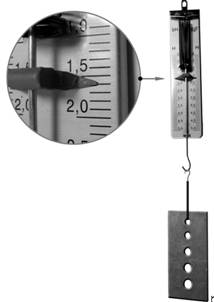
\includegraphics[width=.9\linewidth,height=.48\textheight,keepaspectratio]{_run/photos/4498756fd16b21134650ddd44db86764dbfe98f4a9c2e973429592f86033453e.png}\end{center}\par
\end{center}
}{
\smallskip\noindent\textbf{Решение от GPT}\par
Цена деления динамометра равна $(2{,}0-1{,}5)/5=0{,}1\,\text{Н}$. Указатель показывает $1{,}6\,\text{Н}$; это сила тяжести, уравновешенная силой упругости. С учётом погрешности $F_{\text{тяж}}=(1{,}6\pm0{,}1)\,\text{Н}$.
}

% Source 72C2B7: https://ege.fipi.ru/bank/questions.php?search=1&proj=BA1F39653304A5B041B656915DC36B38&qid=72C2B7
\BankTask{72C2B7}{
При помощи динамометра определяют вес металлической детали. Определите показание динамометра, если погрешность прямого измерения равна цене деления динамометра. Шкала проградуирована в $\text{Н}$.
\begin{center}
\par\begin{center}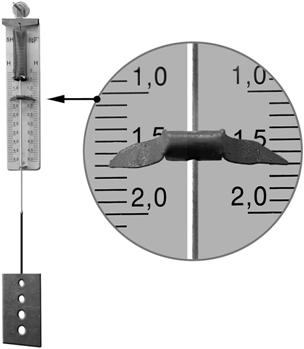
\includegraphics[width=.9\linewidth,height=.48\textheight,keepaspectratio]{_run/photos/1ea90dd9e3195991b9886d0a000478ef743ddaf9eaf6f3a83d7befae3e079b31.png}\end{center}\par
\end{center}
}{
\smallskip\noindent\textbf{Решение от GPT}\par
Между отметками $1{,}0$ и $1{,}5\,\text{Н}$ пять делений, поэтому цена деления равна $0{,}1\,\text{Н}$. Указатель соответствует $1{,}6\,\text{Н}$. Показание с учётом погрешности: $P=(1{,}6\pm0{,}1)\,\text{Н}$.
}

% Source 474F4B: https://ege.fipi.ru/bank/questions.php?search=1&proj=BA1F39653304A5B041B656915DC36B38&qid=474F4B
\BankTask{474F4B}{
При исследовании зависимости давления в газе от температуры ученик измерял температуру в сосуде с газом с помощью термометра. Погрешность измерений температуры равна цене деления шкалы термометра. Чему равна температура газа (в $^{\circ}\text{C}$) по результатам этих измерений?

\par\begin{center}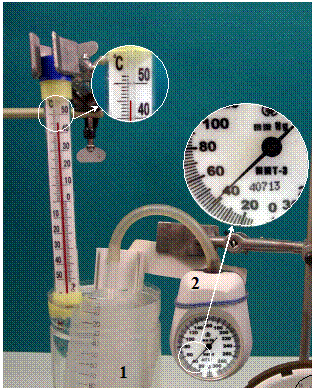
\includegraphics[width=.9\linewidth,height=.48\textheight,keepaspectratio]{_run/photos/dae54c4eae2ecaf531cb3c9cda6a3c4b6b8142f42ce069d29f71e4f49a420283.png}\end{center}\par
}{
\smallskip\noindent\textbf{Решение от GPT}\par
Между отметками $40\,^{\circ}\text{C}$ и $50\,^{\circ}\text{C}$ расположено десять делений, поэтому цена деления равна $1\,^{\circ}\text{C}$. Термометр показывает $48\,^{\circ}\text{C}$, а погрешность равна цене деления. Результат измерения: $t=(48\pm1)\,^{\circ}\text{C}$.
}

% Source E1896D: https://ege.fipi.ru/bank/questions.php?search=1&proj=BA1F39653304A5B041B656915DC36B38&qid=E1896D
\BankTask{E1896D}{
На фотографии изображён спиртовой термометр со шкалой Цельсия. Погрешность измерения температуры при помощи этого термометра равна половине цены деления. Определите абсолютную температуру спирта (в $\text{К}$) в колбе термометра.

\par\begin{center}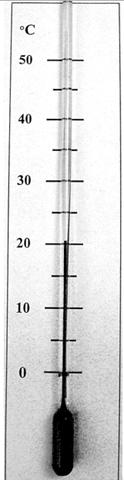
\includegraphics[width=.9\linewidth,height=.48\textheight,keepaspectratio]{_run/photos/5630ecceb8effddffd3091ab131a37434dec32efb2c00debbd378a33ec95d444.png}\end{center}\par
}{
\smallskip\noindent\textbf{Решение от GPT}\par
Термометр показывает $t=20\,^{\circ}\text{C}$, цена деления его шкалы составляет $5\,^{\circ}\text{C}$. Абсолютная температура $T=273+20=293\,\text{К}$, а погрешность $\Delta T=5/2=2{,}5\,\text{К}$. Ответ: $T=(293{,}0\pm2{,}5)\,\text{К}$.
}

% Source e00415: https://ege.fipi.ru/bank/questions.php?search=1&proj=BA1F39653304A5B041B656915DC36B38&qid=e00415
\BankTask{e00415}{
При помощи манометра измеряют давление в баллоне шприца. Запишите показания манометра с учётом абсолютной погрешности измерений, которая равна цене деления манометра. Шкала манометра проградуирована в $\text{мм рт. ст.}$

\par\begin{center}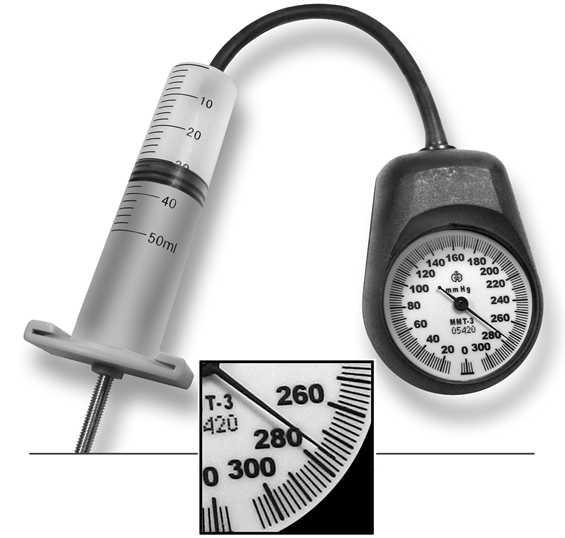
\includegraphics[width=.9\linewidth,height=.48\textheight,keepaspectratio]{_run/photos/a7a66aa8b7b4154db689ccb2c4156b7283e292ee30fee783aa4f403dc6decaf5.png}\end{center}\par
}{
\smallskip\noindent\textbf{Решение от GPT}\par
Между отметками $260\,\text{мм рт. ст.}$ и $280\,\text{мм рт. ст.}$ расположено десять делений, поэтому цена деления равна $2\,\text{мм рт. ст.}$. Стрелка показывает $276\,\text{мм рт. ст.}$; погрешность равна цене деления. Ответ: $p=(276\pm2)\,\text{мм рт. ст.}$.
}

% Source 665C1D: https://ege.fipi.ru/bank/questions.php?search=1&proj=BA1F39653304A5B041B656915DC36B38&qid=665C1D
\BankTask{665C1D}{
На какую величину, согласно показаниям манометра, давление воздуха в баллоне превышает атмосферное давление, если погрешность манометра равна $3\,\text{мм рт. ст.}$?

\par\begin{center}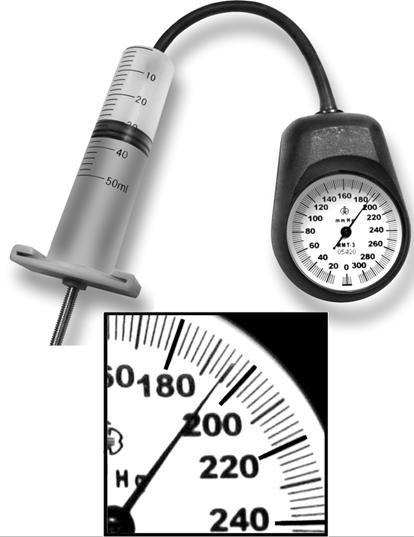
\includegraphics[width=.9\linewidth,height=.48\textheight,keepaspectratio]{_run/photos/1f5975fad0c054eb83a8ec5075afd39d184855df2919034e902c2d44e54ee38f.png}\end{center}\par
}{
\smallskip\noindent\textbf{Решение от GPT}\par
Между отметками $180$ и $200\,\text{мм рт. ст.}$ расположено $10$ делений, поэтому цена деления равна $2\,\text{мм рт. ст.}$. Стрелка показывает избыточное давление $196\,\text{мм рт. ст.}$. С учётом заданной погрешности ответ: $(196\pm3)\,\text{мм рт. ст.}$.
}

% Source A82c5A: https://ege.fipi.ru/bank/questions.php?search=1&proj=BA1F39653304A5B041B656915DC36B38&qid=A82c5A
\BankTask{A82c5A}{
При исследовании зависимости давления газа от температуры ученик измерял давление в сосуде с газом при помощи манометра. Шкала манометра проградуирована в миллиметрах ртутного столба. Абсолютная погрешность измерения давления равна половине цены деления шкалы манометра. Каково показание манометра с учётом погрешности измерения?

\par\begin{center}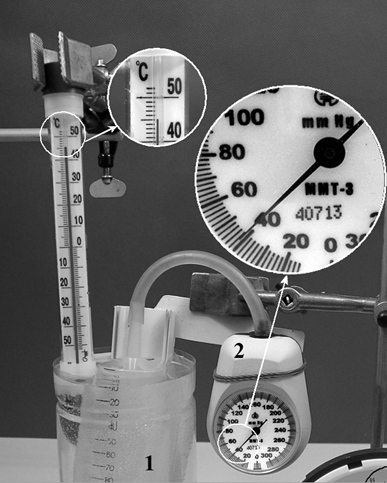
\includegraphics[width=.9\linewidth,height=.48\textheight,keepaspectratio]{_run/photos/b7a3d0db007ac02857bf8446cefca5ec387373d7ff396a9c5eb1ea0f10be8eb7.png}\end{center}\par
}{
\smallskip\noindent\textbf{Решение от GPT}\par
Стрелка манометра показывает $40\,\text{мм рт. ст.}$. Цена деления шкалы равна $2\,\text{мм рт. ст.}$, поэтому абсолютная погрешность составляет $\Delta p=1\,\text{мм рт. ст.}$. Ответ: $(40\pm1)\,\text{мм рт. ст.}$.
}

% Source 9BB8D9: https://ege.fipi.ru/bank/questions.php?search=1&proj=BA1F39653304A5B041B656915DC36B38&qid=9BB8D9
\BankTask{9BB8D9}{
В паспорте барометра указано, что абсолютная погрешность прямого измерения давления равна $3\,\text{гПа}$.

Определите показания барометра.

\par\begin{center}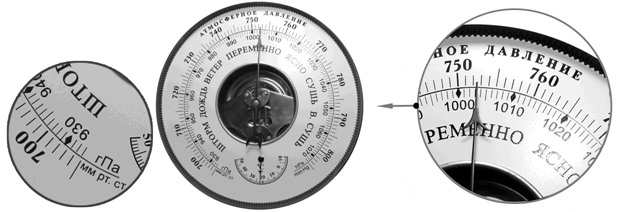
\includegraphics[width=.9\linewidth,height=.48\textheight,keepaspectratio]{_run/photos/8ba6dfb379d477455dadbbc062874489dbd6d8840a85a640f650b079d54d40d9.png}\end{center}\par
}{
\smallskip\noindent\textbf{Решение от GPT}\par
Показание считываем по шкале, проградуированной в гектопаскалях. Цена её деления равна $2\,\text{гПа}$, стрелка показывает $1002\,\text{гПа}$. С учётом паспортной погрешности ответ: $(1002\pm3)\,\text{гПа}$.
}

% Source AF97AC: https://ege.fipi.ru/bank/questions.php?search=1&proj=BA1F39653304A5B041B656915DC36B38&qid=AF97AC
\BankTask{AF97AC}{
Запишите показания барометра с учётом абсолютной погрешности измерений. Верхняя шкала барометра проградуирована в $\text{кПа}$, нижняя – в $\text{мм рт. ст.}$ Абсолютная погрешность прямого измерения барометра равна цене деления барометра.

\par\begin{center}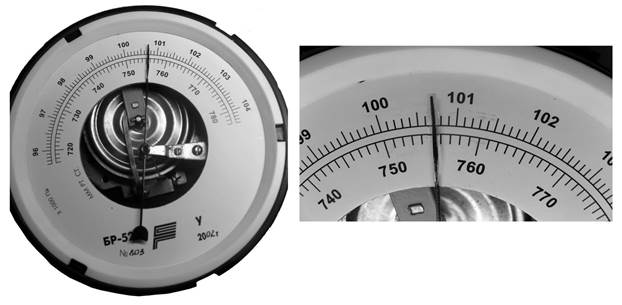
\includegraphics[width=.9\linewidth,height=.48\textheight,keepaspectratio]{_run/photos/11a36f0ad1c8da0340896ec0c60d1a49444651ea2932fa68881be2c80c9dfc68.png}\end{center}\par
}{
\smallskip\noindent\textbf{Решение от GPT}\par
На нижней шкале между отметками $750$ и $760\,\text{мм рт. ст.}$ десять делений, поэтому цена деления равна $1\,\text{мм рт. ст.}$ Стрелка показывает $755\,\text{мм рт. ст.}$, следовательно, результат измерения: $p=(755\pm1)\,\text{мм рт. ст.}$
}

% Source ECB765: https://ege.fipi.ru/bank/questions.php?search=1&proj=BA1F39653304A5B041B656915DC36B38&qid=ECB765
\BankTask{ECB765}{
С помощью барометра проводились измерения атмосферного давления. Верхняя шкала барометра проградуирована в килопаскалях, а нижняя шкала — в миллиметрах ртутного столба (см. рисунок). Погрешность измерений давления равна цене деления шкалы барометра. Чему равно атмосферное давление в килопаскалях по результатам этих измерений?

\par\begin{center}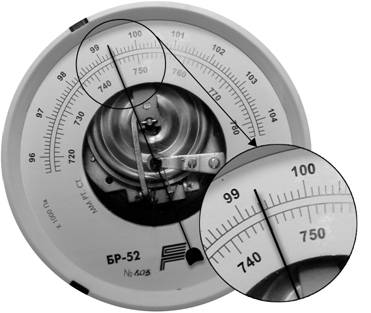
\includegraphics[width=.9\linewidth,height=.48\textheight,keepaspectratio]{_run/photos/d7816d1a43a65c6820b9b93bca60a8925d0c3609574e33f709f86e9d456c7467.png}\end{center}\par
}{
\smallskip\noindent\textbf{Решение от GPT}\par
Между отметками $99$ и $100\,\text{кПа}$ десять делений, поэтому цена деления и абсолютная погрешность равны $0{,}1\,\text{кПа}$. Стрелка показывает $99{,}4\,\text{кПа}$, следовательно, $p=(99{,}4\pm0{,}1)\,\text{кПа}$.
}

% Source 104711: https://ege.fipi.ru/bank/questions.php?search=1&proj=BA1F39653304A5B041B656915DC36B38&qid=104711
\BankTask{104711}{
Чему равна сила тока в лампочке (см. рисунок), если погрешность прямого измерения силы тока амперметром на пределе измерения $3\,\text{А}$ равна $\Delta I_{1}=0{,}15\,\text{А}$, а на пределе измерения $0{,}6\,\text{А}$ равна $\Delta I_{2}=0{,}03\,\text{А}$?

\par\begin{center}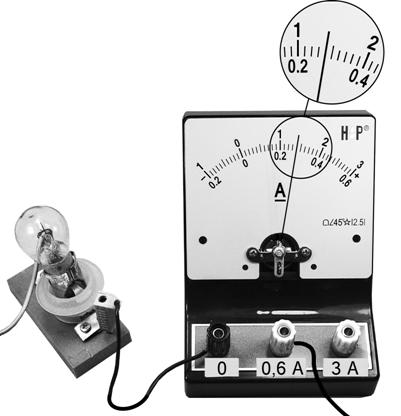
\includegraphics[width=.9\linewidth,height=.48\textheight,keepaspectratio]{_run/photos/743589c7a25f4626fef32516fe988e2f9a3aaf9e716085925fe646d261a361c9.png}\end{center}\par
}{
\smallskip\noindent\textbf{Решение от GPT}\par
Провода подключены к клеммам $0$ и $0{,}6\,\text{А}$, поэтому показания читаем по шкале с пределом $0{,}6\,\text{А}$. Цена её деления равна $0{,}02\,\text{А}$, а стрелка показывает $0{,}28\,\text{А}$. Для выбранного предела $\Delta I=0{,}03\,\text{А}$, поэтому $I=(0{,}28\pm0{,}03)\,\text{А}$.
}

% Source 8B7A2B: https://ege.fipi.ru/bank/questions.php?search=1&proj=BA1F39653304A5B041B656915DC36B38&qid=8B7A2B
\BankTask{8B7A2B}{
Чему равно напряжение на лампочке (см. рисунок), если погрешность прямого измерения напряжения на пределе измерения $3\,\text{В}$ равна $\pm0{,}15\,\text{В}$, а на пределе измерения $6\,\text{В}$ равна $\pm0{,}25\,\text{В}$?
\par\par\begin{center}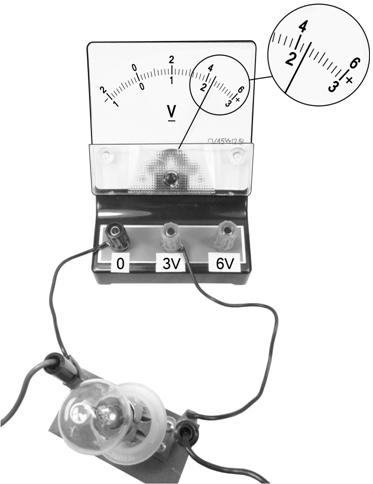
\includegraphics[width=.9\linewidth,height=.48\textheight,keepaspectratio]{_run/photos/ce06b83c7bc39257530becc0e64a3fda1ec8a0fdbf50b68b690f4118c0069bf7.png}\end{center}\par
}{
\smallskip\noindent\textbf{Решение от GPT}\par
Провода подключены к клеммам $0$ и $3\,\text{В}$, поэтому показание считываем по шкале с пределом $3\,\text{В}$. Стрелка показывает $2{,}2\,\text{В}$, а погрешность на этом пределе составляет $0{,}15\,\text{В}$. Ответ: $U=(2{,}20\pm0{,}15)\,\text{В}$.
}

% Source 9503F7: https://ege.fipi.ru/bank/questions.php?search=1&proj=BA1F39653304A5B041B656915DC36B38&qid=9503F7
\BankTask{9503F7}{
Определите показания миллиамперметра (см. рисунок), если абсолютная погрешность прямого измерения силы тока равна цене деления миллиамперметра.
\par\par\begin{center}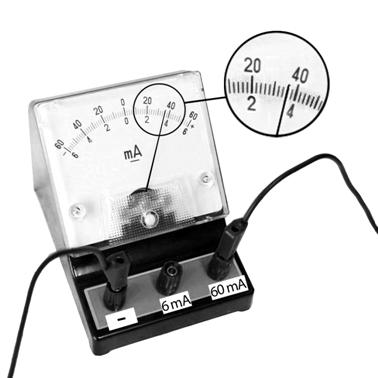
\includegraphics[width=.9\linewidth,height=.48\textheight,keepaspectratio]{_run/photos/2632b2416f1bc8ef557d07e8c1174ca9aa69f7f9adce45d3d5e1e10ae32bf559.png}\end{center}\par
}{
\smallskip\noindent\textbf{Решение от GPT}\par
Миллиамперметр подключён к клемме с пределом измерения $60\,\text{мА}$. Между отметками $20\,\text{мА}$ и $40\,\text{мА}$ расположено $10$ делений, поэтому цена деления равна $2\,\text{мА}$. Стрелка показывает $36\,\text{мА}$, следовательно, $I=(36\pm2)\,\text{мА}$.
}

% Source 32781A: https://ege.fipi.ru/bank/questions.php?search=1&proj=BA1F39653304A5B041B656915DC36B38&qid=32781A
\BankTask{32781A}{
Ученик собрал электрическую цепь, состоящую из батарейки ($1$), реостата ($2$), ключа ($3$), амперметра ($4$) и вольтметра ($5$). После этого он провёл измерения напряжения на источнике и силы тока в цепи. Абсолютная погрешность измерения силы тока в цепи и напряжения на источнике равна половине цены деления амперметра и вольтметра. Чему равно по результатам этих измерений напряжение на клеммах батарейки?
\par\par\begin{center}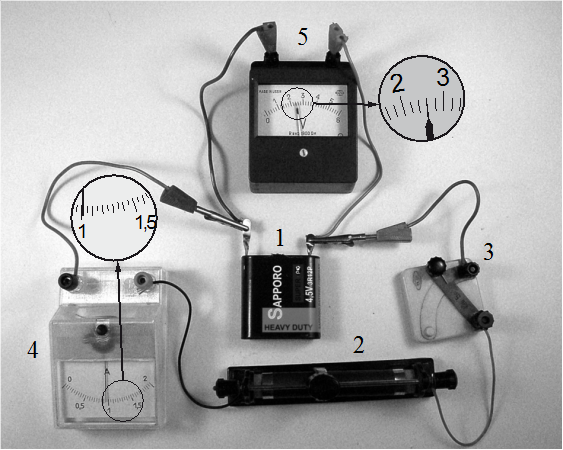
\includegraphics[width=.9\linewidth,height=.48\textheight,keepaspectratio]{_run/photos/15846bb727f4595f7efe37d007146f1203b4b0a0b18d4809b44a8816aa4faa9a.png}\end{center}\par
}{
\smallskip\noindent\textbf{Решение от GPT}\par
По шкале вольтметра напряжение равно $2{,}8\,\text{В}$. Цена деления составляет $0{,}2\,\text{В}$, поэтому абсолютная погрешность $\Delta U=0{,}2/2=0{,}1\,\text{В}$. Ответ: $U=(2{,}8\pm0{,}1)\,\text{В}$.
}

% Source EB5EC2: https://ege.fipi.ru/bank/questions.php?search=1&proj=BA1F39653304A5B041B656915DC36B38&qid=EB5EC2
\BankTask{EB5EC2}{
На рисунке приведена фотография электрической цепи при измерении сопротивления реостата. Погрешности измерения приборами силы тока и напряжения равны цене деления амперметра и вольтметра. Каковы по результатам этих измерений показания вольтметра с учётом погрешности измерения?

\par\begin{center}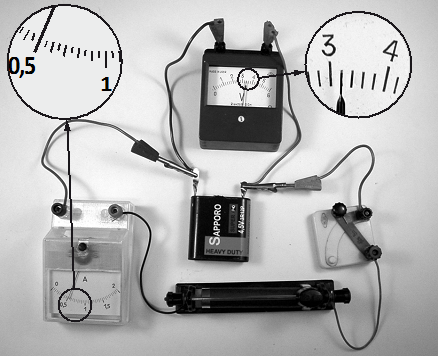
\includegraphics[width=.9\linewidth,height=.48\textheight,keepaspectratio]{_run/photos/940f8bf4e55206f33ae482b15a1a887c4a29e37bb52f41c6b03deec7dda397d2.png}\end{center}\par
}{
\smallskip\noindent\textbf{Решение от GPT}\par
Между отметками $3\,\text{В}$ и $4\,\text{В}$ расположено пять делений, поэтому цена деления вольтметра равна $0{,}2\,\text{В}$. Стрелка показывает $3{,}2\,\text{В}$; по условию погрешность равна цене деления. Ответ: $U=(3{,}2\pm0{,}2)\,\text{В}$.
}

% Source 0C0F85: https://ege.fipi.ru/bank/questions.php?search=1&proj=BA1F39653304A5B041B656915DC36B38&qid=0C0F85
\BankTask{0C0F85}{
Ученик собрал электрическую цепь, состоящую из батарейки, двух резисторов, амперметра и вольтметра. После этого он провёл измерения напряжения на одном из резисторов и силы тока в цепи. Погрешности измерения силы тока в цепи и напряжения на источнике равны цене деления амперметра и вольтметра. Чему равно по результатам этих измерений напряжение на резисторе $R_{1}$? Вольтметр проградуирован в вольтах ($\text{В}$).

\begin{center}
\begin{tikzpicture}[book diagram,x=0.024cm,y=-0.024cm,line width=0.7pt]
\draw (98,28)--(130,28);
\draw (130,13) rectangle (206,42);
\node at (168,27) {$R_1$};
\draw (206,28)--(274,28);
\draw (274,13) rectangle (350,42);
\node at (312,27) {$R_2$};
\draw (350,28)--(375,28)--(375,73);
\draw (375,96) circle (23);
\node at (375,96) {$\mathrm A$};
\draw (375,119)--(375,162)--(241,162);
\draw[line width=1.4pt] (230,148)--(230,176);
\draw[line width=2.5pt] (239,153)--(239,171);
\draw (230,162)--(98,162)--(98,28);
\node at (262,143) {$\mathcal E,\,r$};
\draw (239,28)--(239,104)--(194,104);
\draw (98,104)--(147,104);
\draw (170.5,104) circle (23.5);
\node at (170.5,104) {$\mathrm V$};
\fill (98,104) circle (3);
\fill (239,28) circle (3);
\draw (32,100) circle (31);
\draw[-{book tip},line width=0.5pt] (159,81) to[out=220,in=-40] (47,75);
\begin{scope}[shift={(32,106)},rotate=22]
\foreach \i in {-4,-3,...,4} {
  \draw[line width=0.45pt] ({6*\i},-5)--({6*\i},5);
}
\draw[line width=0.65pt] (-12,-8)--(-12,6);
\draw[line width=0.65pt] (18,-8)--(18,6);
\node[font=\small] at (-12,-16) {$4$};
\node[font=\small] at (18,-16) {$5$};
\draw[line width=1.15pt] (4,25)--(6,-8);
\end{scope}
\draw (481,124) circle (48);
\draw[-{book tip},line width=0.5pt] (389,78) to[out=-62,in=-120] (458,82);
\begin{scope}[shift={(479,114)},rotate=22]
\foreach \i in {-16,-15,...,16} {
  \draw[line width=0.4pt] ({2*\i},-4)--({2*\i},3);
}
\foreach \i in {-8,-6,-4,-2,0,2,4,6,8} {
  \draw[line width=0.5pt] ({4*\i},-7)--({4*\i},5);
}
\draw[line width=0.6pt] (-20,-9)--(-20,7);
\draw[line width=0.6pt] (20,-9)--(20,7);
\node[font=\small] at (-20,19) {$0{,}2$};
\node[font=\small] at (20,19) {$0{,}4$};
\end{scope}
\draw[line width=1.15pt] (470,118)--(487,79);
\end{tikzpicture}
\end{center}
}{
\smallskip\noindent\textbf{Решение от GPT}\par
Вольтметр подключён параллельно резистору $R_1$ и измеряет напряжение на нём. Между отметками $4\,\text{В}$ и $5\,\text{В}$ пять делений, поэтому цена деления составляет $0{,}2\,\text{В}$, а показание прибора — $4{,}6\,\text{В}$. Погрешность равна цене деления: $U_1=(4{,}6\pm0{,}2)\,\text{В}$.
}

\end{document}
